\frontmatter
% ---------------- cover
\thispagestyle{empty}
\AddToShipoutPictureBG*{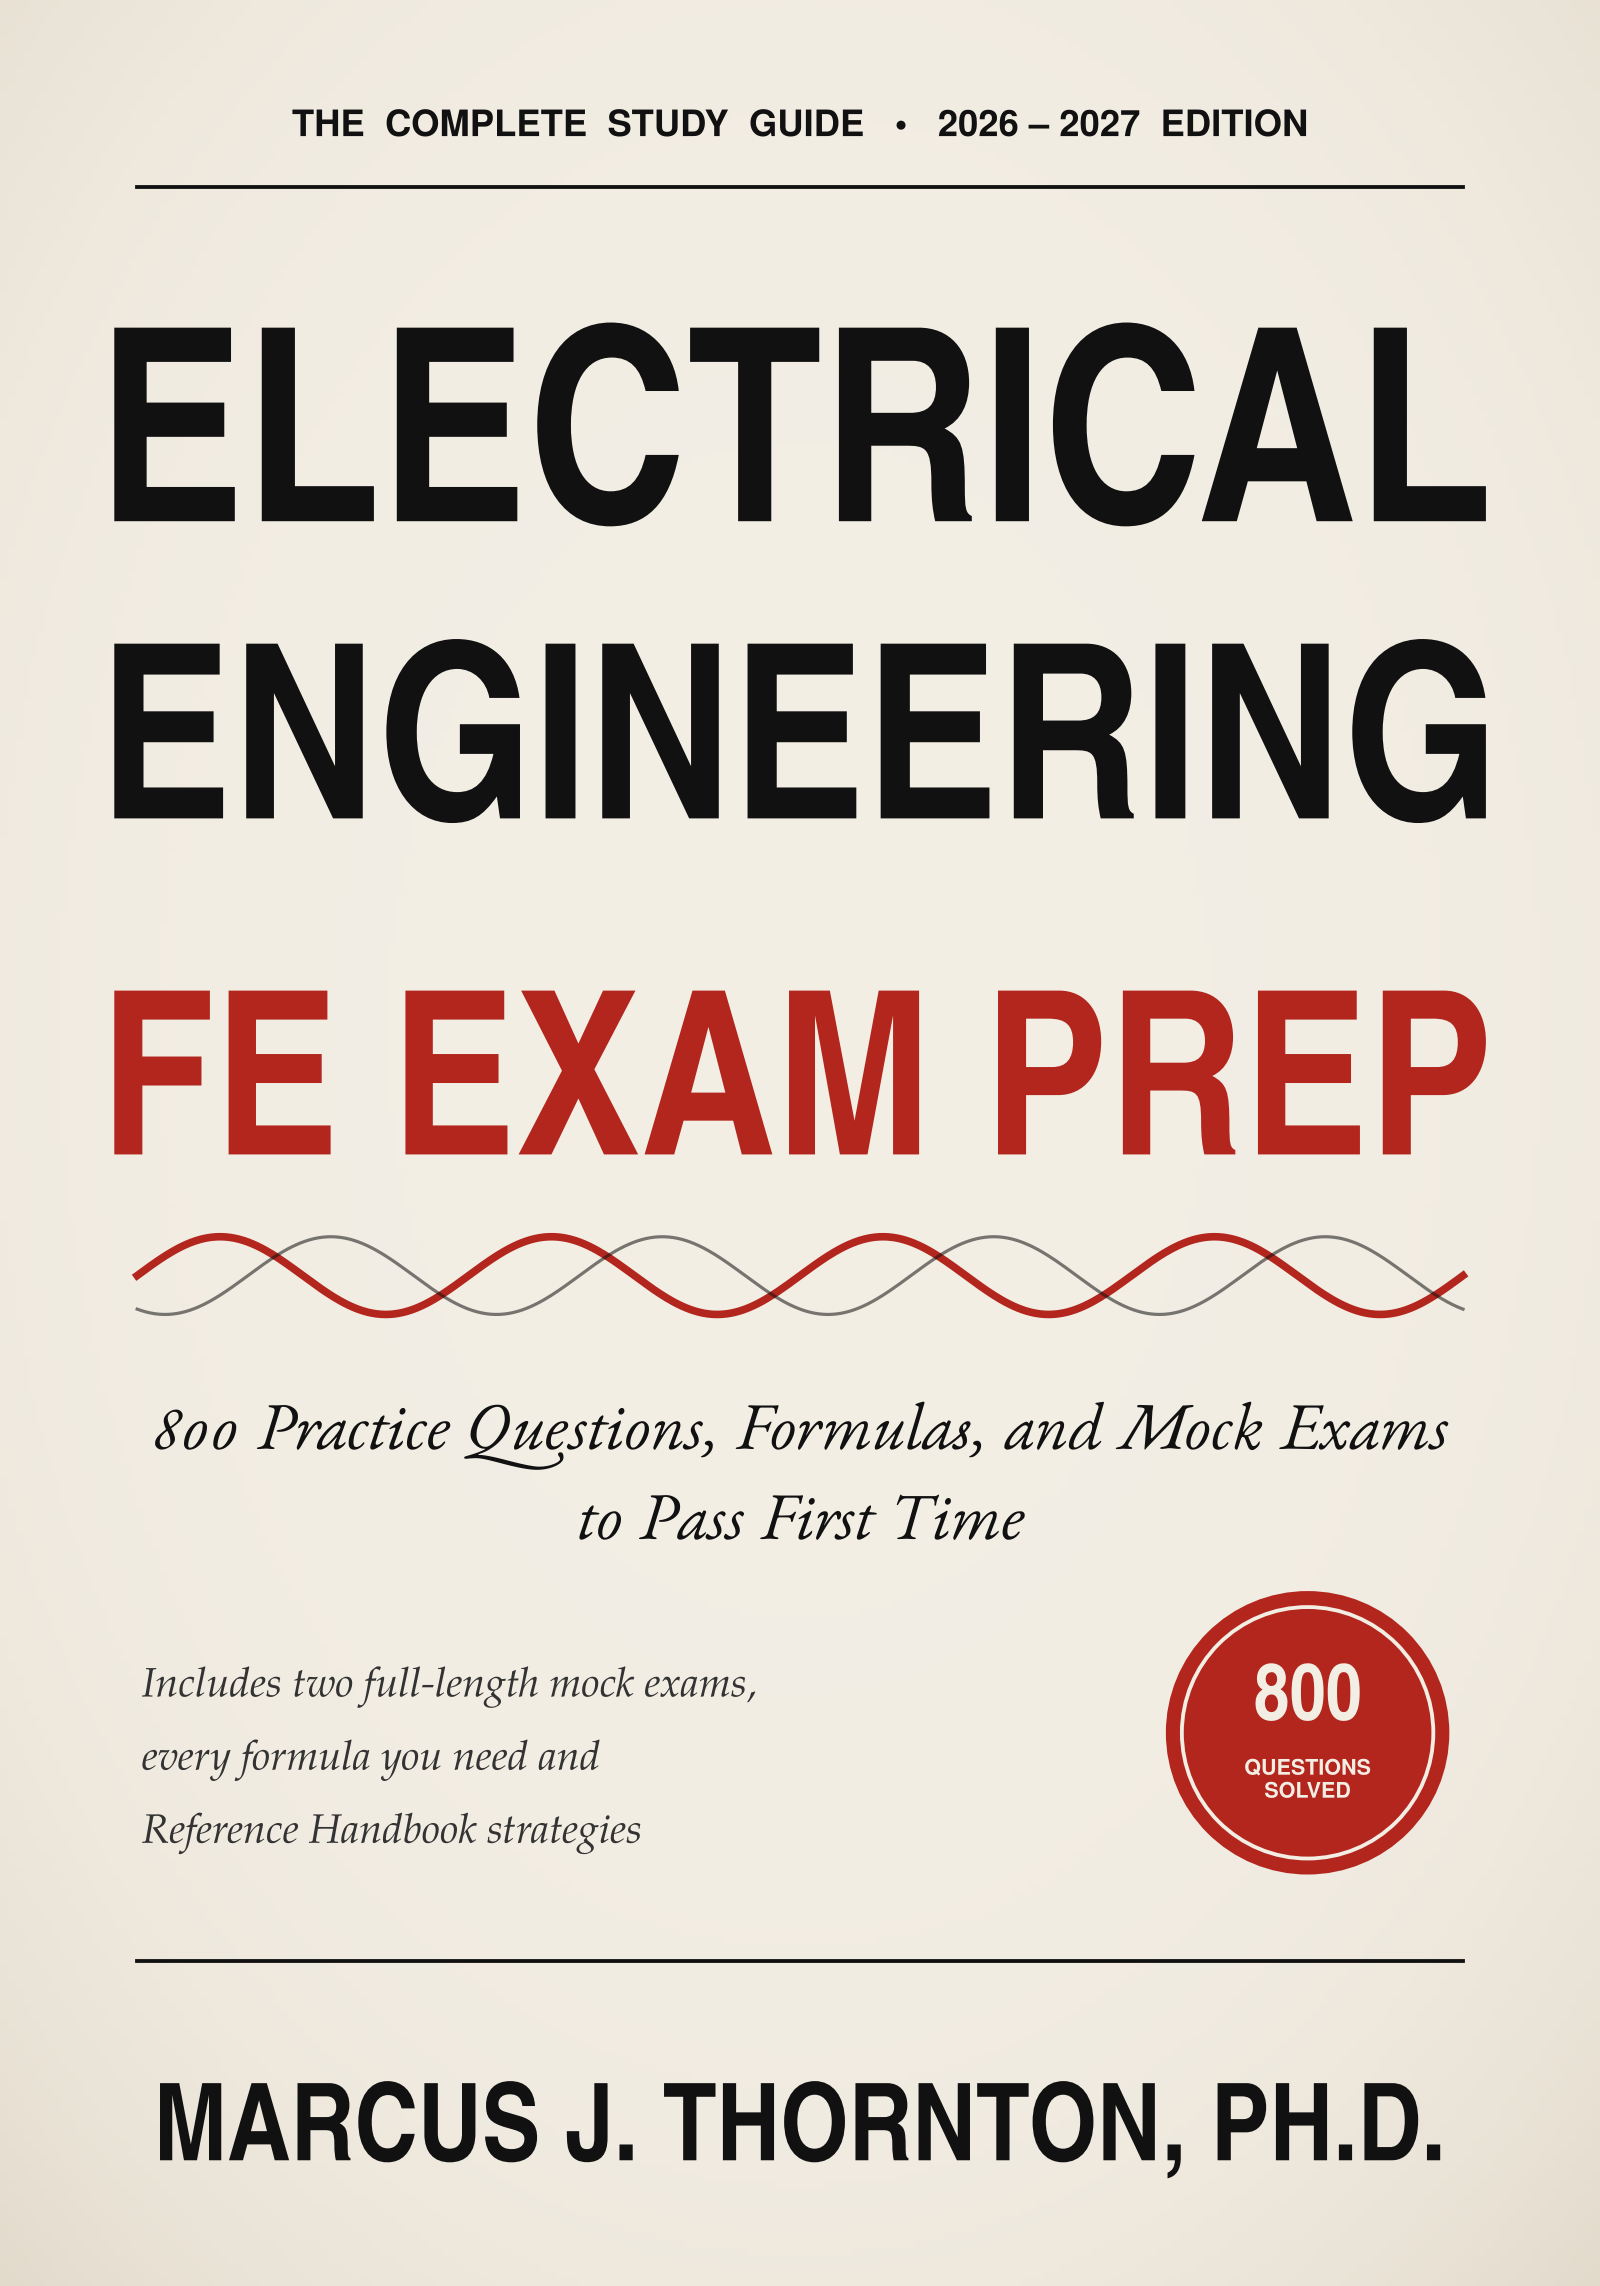
\includegraphics[width=\paperwidth,height=\paperheight]{figures/cover.png}}
\mbox{}
\clearpage
\thispagestyle{empty}\mbox{}\clearpage
% ---------------- half title
\thispagestyle{empty}
\vspace*{0.3\textheight}
\begin{center}
{\fontsize{22}{28}\selectfont\color{inkblue}\bfseries Electrical Engineering\\[4pt] FE Exam Prep 2026--2027\par}
\vspace{14pt}{\color{copper}\rule{0.25\textwidth}{0.8pt}}
\end{center}
\clearpage
\thispagestyle{empty}\mbox{}\clearpage
% ---------------- title page
\thispagestyle{empty}
\vspace*{0.12\textheight}
\begin{center}
{\addfontfeature{LetterSpace=30}\large\scshape\color{copper}The Complete Study Guide\par}
\vspace{22pt}
{\fontsize{34}{40}\selectfont\bfseries\color{inkblue}Electrical Engineering\\[6pt]FE Exam Prep\\[6pt]2026--2027\par}
\vspace{18pt}
{\color{copper}\rule{0.35\textwidth}{0.9pt}}\par
\vspace{18pt}
{\Large\itshape\color{inkblue}800 Practice Questions, Formulas, and Mock Exams\\[2pt] to Pass First Time\par}
\vfill
{\addfontfeature{LetterSpace=20}\Large\scshape\color{inkblue}Marcus J. Thornton, Ph.D.\par}
\vspace{0.08\textheight}
\end{center}
\clearpage
% ---------------- copyright
\thispagestyle{empty}
\vspace*{\fill}
{\small\raggedright
\textbf{Electrical Engineering FE Exam Prep 2026--2027:\\ The Complete Study Guide}\\
800 Practice Questions, Formulas, and Mock Exams to Pass First Time\\[10pt]
Copyright \textcopyright\ 2026 by Marcus J. Thornton, Ph.D.\\
All rights reserved.\\[10pt]
No part of this publication may be reproduced, stored in a retrieval system or transmitted in any form or by any means---electronic, mechanical, photocopying, recording or otherwise---without the prior written permission of the author, except for brief quotations in critical reviews and certain other non-commercial uses permitted by copyright law.\\[10pt]
FE, Fundamentals of Engineering and NCEES are trademarks or registered trademarks of the National Council of Examiners for Engineering and Surveying. This book is an independent study guide. It is not endorsed by, sponsored by or affiliated with NCEES or any state licensing board. Examination specifications, policies and the content of the \emph{FE Reference Handbook} change from time to time; always confirm current details at the official NCEES website before you register and before you sit the exam.\\[10pt]
Every effort has been made to ensure the accuracy of the material in this book. The author and publisher accept no responsibility for errors or omissions, or for any loss arising from the use of the information it contains. The practice questions are original works written for study purposes and are not taken from any actual examination.\\[10pt]
First edition, 2026\\[10pt]
Typeset in TeX Gyre Pagella.\\
}
\clearpage
% ---------------- dedication
\thispagestyle{empty}
\vspace*{0.3\textheight}
\begin{center}
{\itshape\large\color{inkblue}For every engineer who has sat at a kitchen table at midnight,\\ working one more problem.\\[8pt] This one is for you.\par}
\end{center}
\clearpage
\thispagestyle{empty}\mbox{}\clearpage
